\section{Stima intervallare}

\subsection{Credibility intervall (bayesiano) e Confidence interval (frequentista)}

\begin{frame}[fragile]{Bayesian credibility Interval}
\begin{block}{Credibility (della posterior)}
\begin{align*}
&\cred{(x)}=\int_{\mu\in\inf(x)}\Pi(\mu|x)\,d\mu=\int_{\mu\inf(x)}\frac{\prob{(x|\mu)}\prob{(\mu)}}{\int\,d\mu}\,d\mu>\cl{}\\
&
\end{align*}
\end{block}
\begin{block}{Ordinamento}
\begin{picture}(100,130)
\put(20,20){
\begin{tikzpicture}[scale=0.4]
\def\basefunc{exp(-(x-1)^2)}
        \begin{axis}[title={central},name=central,samples=50,ymin=0,xmin=-2,xmax=4,xlabel={$m$},ylabel={$\prob{(m|x_0)}$}]
        \addplot gnuplot [no marks,domain={-2:0}]{\basefunc} \closedcycle; 
        \addplot gnuplot [no marks,domain={2:4}]{\basefunc} \closedcycle; 
        \addplot gnuplot [black,thick,fill=grey,smooth,no marks,domain={0:2}]{\basefunc} \closedcycle;
        \node (unomenocl) at (axis cs:-1,0.3) {$1-\frac{\alpha}{2}$};
        \end{axis}
        \begin{axis}[title={upper limit}, at={($(central)+(4.5cm,-3cm)$)},name=upper,samples=50,ymin=0,xmin=-2,xmax=4,xlabel={$m$},ylabel={$\prob{(m|x_0)}$}]
        \addplot gnuplot [no marks,fill=grey,domain={-2:2}]{\basefunc} \closedcycle; 
        \addplot gnuplot [black,thick,smooth,no marks,domain={2:4}]{\basefunc};   
        \end{axis}
        \edef\oprob{0.47}
        \begin{axis}[at={($(upper)+(4.5cm,-3cm)$)}, title={probability order},name=central,samples=50,ymin=0,xmin=-2,xmax=4,xlabel={$m$},ylabel={$\prob{(m|x_0)}$}]
        \addplot[name path=prob] gnuplot[grey,thick,smooth,no marks]{\oprob};
        \addplot[name path=gauss] gnuplot[black,thick,smooth,no marks]{\basefunc};
        \path [name intersections={of=gauss and prob ,by={Pa,Pb}}];
        \node[above left] at (Pa) {$x_-$} node[above right] at (Pb) {$x_+$};
        \pgfkeys{/pgf/fpu=true}
        \pgfmathparse{1-sqrt(-ln(\oprob))}
        \def\xleft{\pgfmathresult}
        \pgfmathparse{1+sqrt(-ln(\oprob))}
        \def\xright{\pgfmathresult}
        \pgfmathparse{1+sqrt(-ln(\oprob))}
        \pgfkeys{/pgf/fpu=false}
        \addplot gnuplot [no marks,fill=grey,domain={0.13:1.87}]{\basefunc} \closedcycle; 
        \node (unomenocl) at (axis cs:0,0.7) {$CL$};
        \end{axis}
    \end{tikzpicture}}
\end{picture}
\end{block}
\end{frame}

\begin{frame}{Neyman construction. Frequentist confidence intervals}
%reminder: banda confidenza con pgfplot/gnuplot
\begin{columns}[T]
\begin{column}{0.4\textwidth}
\begin{figure}
    \centering
    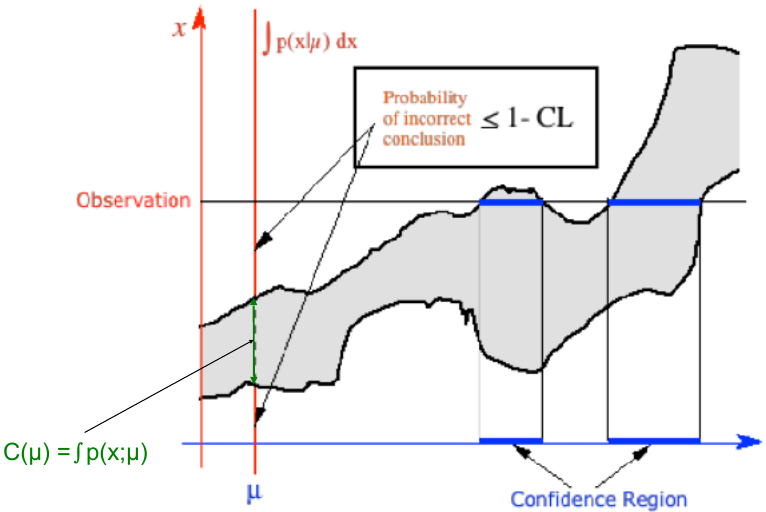
\includegraphics[width=0.9\textwidth,keepaspectratio]{clband}
    \label{fig:clband}
\end{figure}
\begin{figure}
    \centering
    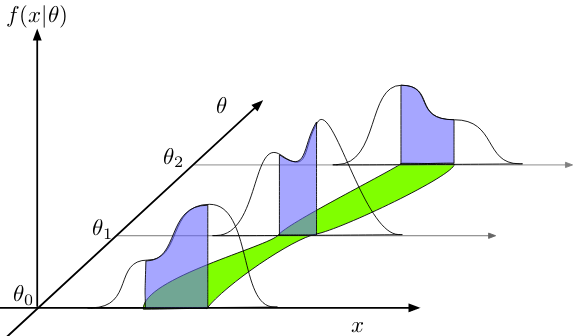
\includegraphics[width=0.9\textwidth,keepaspectratio]{neyman}
    \label{fig:neyman}
\end{figure}
\end{column}
\begin{column}{0.6\textwidth}
\begin{block}{Costruzione di Neyman}
Coverage: $\coverage{(\mu)}=\int_{x:\mu\in f(x)}\prob{(x:\mu)}\,dx$, $f(x)$ associa un intervallo nello spazio dei parametri a una misura; l'algoritmo ha livello di confidenza $\cl=\inf_{\mu\in A}C(\mu)$ cio\'e l'intervallo associato alla data misura ha probabilit\'a $\cl{}$ di contenere il parametro.
\end{block}
\begin{block}{Ordering}
''The way I integrate over the data''
\end{block}
\end{column}
\end{columns}
\end{frame}

\begin{frame}{Feldman-Cousins unified approach.}
\begin{columns}[T]
\begin{column}{0.5\textwidth}
insactisfaction with Neyman construction for upper limit in case of empty/unphysical interval (flip-flop problem depending on data)
\end{column}
\begin{column}{0.5\textwidth}
LR-ordering $R=\frac{\prob{(x;\mu)}}{\prob{(x;\mu_{best})}}$: values of x/n are added to acceptance region as decreasing function of R.
\end{column}
\end{columns}
\end{frame}

\subsection{Pivotal quantities}

\begin{frame}{Pivot}
Pivot: RV $U(T,\theta)$ funzione dib statistica sufficiente e parametro ma la distribuzione di U non dipende dal parametro $\forall \theta\in\Theta$ (asymptotic if true for $n\to\infty$).
\begin{align*}
&p(x;\mu)=\frac{1}{\sqrt{2\pi}\sigma}\exp{-\frac{(x-\mu)^2}{2\sigma^2}}\\
&(s=\frac{x-\mu}{\sigma}:\ p(s;\mu)=N(0,1)\\
&\int_{s>c}p(s)\,DS=\cl{}
\end{align*}
\mykeyword{Pivot. 2-sided CI for exponential}:
\begin{align*}
&f(x;\theta)=\invers{\theta}\exp{-\frac{x}{\theta}}I(x>0)\ \to\ g(u)=\exp{-u}I(u>0)\\
&\prob{(a<u<b)}=1-\alpha\Rightarrow\prob{(\theta\in(\invers{b}x,\invers{a}x))}=1-\alpha\ (\alpha\leftrightarrow1-\alpha)\\
&
\end{align*}
\end{frame}

\begin{frame}{Teorema di Wilks}
$p(x;\mu)$ due volte differenziabile con dominio indipendente da parametro $\Omega(x;\mu)=\Omega(x)$: \[\lambda(x;\mu)=2\log{[\frac{\sup_{\mu}{p(x;\mu)}}{p(x;\mu)}]}\] (log-likelihood ratio statistics) ha asintoticamente pdf universale e indipendente da $\mu$: distribuzione di $\chi^2$ con dof pari a dimensione di $\vec{\mu}$.
\begin{align*}
&\ln{L(\theta)}-\ln{L(\hat{\theta})}=-\frac{1}{2}\invers{F}_{\chi_n^2}(1-\alpha)
\end{align*}
\end{frame}

\begin{wordonframe}{Esempi intervalli di confidenza e credibilit\'a}
\begin{block}{Limite superiore Poisson con $k=0$}
$\prob{(k|\mu)}=\frac{\mu^k\exp{-\mu}}{k!}$: registro $k=0$ conteggi, ricavo limite superiore frequentista e bayesiano per $\mu$
\end{block}

\mykeyword{Ex: limite superiore bayesiano per Poisson} - La posterior $\prob{(\mu|0)}=\exp{-\mu}$ per $\cl{}=\alpha\%$ si ha $\int_0^{\mu_u}\exp{-\mu}\,d\mu=\alpha$, per $\cl{}=90\%$ si ha $\mu<2.3@90\%\cl{}$.
\begin{columns}[T]
\begin{column}{0.5\textwidth}
\mykeyword{Ex: limite superiore frequentista per Poisson} - Upper limit: $\sum_{k_{min}}^{\infty}\prob{(k|\mu)}=\alpha$; $\prob{(0|\mu)}=0.1 (=1-\alpha)$ per $\mu_0=\ln{10}$, $\prob{(0|\mu_1)}+\prob{(1|\mu_1)}=0.1$ per $\mu_1=3.89$, $\prob{(0|\mu_1)}+\prob{(1|\mu_1)}+\prob{(2|\mu_1)}=0.1$ per $\mu_2=5.32$
\end{column}
\begin{column}{0.5\textwidth}
\begin{picture}(100,130)
\put(20,20){
	\begin{tikzpicture}[scale=0.4]
	\begin{axis}[title={Coverage},name=central,samples=50,ymin=0,xmin=0,xmax=6,xlabel={$\mu$},ylabel={$k$},y label style={rotate=-90, at={(-0.1,1.)}},extra x ticks={2.3,3.89,5.32},extra x tick style={% changes for extra x ticks
		tick label style={yshift=-4mm}},
	extra x tick labels={$\mu_0$, $\mu_1$, $\mu_2$},extra y ticks={0},extra y tick labels={measure $k=0$}]
	\addplot+[name path=dwcover,const plot, no marks, thick] coordinates {(0,0) (2.3,1) (3.89,2) (5.32,3)};
	\addplot[quiver={u=0,v=x>2.3 ? (x>3.9 ? -1 : -2):-3},-stealth, samples=15] {3}; 
	\end{axis}
	\end{tikzpicture}}
\end{picture}	
\end{column}
\end{columns}

\mykeyword{Ex: Poisson con $k=0,1,2$ conteggi e ordinamento LR, Up, Down, Central} -

\mykeyword{Ex: Limiti bayesiani e frequentisti sul numero di facce dadi D\&D estrazioni 1,1} - $S=\{4,6,8,10,12,20\}$:
\begin{columns}[T]
\begin{column}{0.5\textwidth}
 \mykeyword{T bayes (lancio 6 dadi)} $\pgfkeys{/pgf/fpu=true}\prob{(1)}=\sum_i\prob{(D_i)}\prob{(1|D_i)}=\xdef\Sum{0}
\foreach \i in {4,6,8,10,12,20} {\xdef\Sum{\Sum+1/(6*\i)}}\pgfmathparse{\Sum}\pgfmathprintnumber{\pgfmathresult}\pgfkeys{/pgf/fpu=false}$
Limite superiore al numero di facce: $\sum_{\mu}\prob{(x_0;\mu)}\geq1-\alpha$, $n_f\leq12$ at $\cl>90\%$
\end{column}
\begin{column}{0.5\textwidth}
\pgfkeys{/pgf/fpu=true}
\pgfmathparse{(1/4)*(1/6)*(1/0.1292)}\pgfmathsetmacro{\postfour}{\pgfmathresult}
\pgfmathparse{(1/6)*(1/6)*(1/0.1292)}\pgfmathsetmacro{\postsix}{\pgfmathresult}
\pgfmathparse{(1/8)*(1/6)*(1/0.1292)}\pgfmathsetmacro{\posteight}{\pgfmathresult}
\pgfmathparse{(1/10)*(1/6)*(1/0.1292)}\pgfmathsetmacro{\postten}{\pgfmathresult}
\pgfmathparse{(1/12)*(1/6)*(1/0.1292)}\pgfmathsetmacro{\posttwelve}{\pgfmathresult}
\pgfmathparse{(1/20)*(1/6)*(1/0.1292)}\pgfmathsetmacro{\posttwenty}{\pgfmathresult}
\pgfkeys{/pgf/fpu=false}
\begin{tikzpicture}[scale=0.5]
\begin{axis}[
ybar stacked,
bar width=15pt,
nodes near coords% = {%
%\pgfmathprintnumberto[fixed,assume math mode=true]{\pgfplotspointmeta}{\myval}%
%\pgfmathparse{\myval<0.05?:\myval}\pgfmathresult%}
,
enlargelimits=0.2,
ylabel={$\prob{(D_i|1)}$},
symbolic x coords={d4, d6, d8, d10, d12, d20},
xtick=data,
x tick label style={anchor=north},
xticklabels={$D_4$, $D_6$, $D_8$, $D_{10}$, $D_{12}$, $D_{20}$},cycle list name = ColorListBar
]
\addplot+[ybar] plot coordinates {(d4,\postfour) (d6,\postsix) (d8,\posteight) (d10,\postten) (d12,\posttwelve) (d20,\posttwenty)};
\end{axis}
\end{tikzpicture}
Probability ordering (Cosa vuol dire ordinamento?)
\end{column}
\end{columns}
\begin{columns}[T]
	\begin{column}{0.5\textwidth}
\begin{tikzpicture}[scale=0.3]
\begin{axis}[
ybar stacked,
bar width=15pt,
nodes near coords% = {%
%\pgfmathprintnumberto[fixed,assume math mode=true]{\pgfplotspointmeta}{\myval}%
%\pgfmathparse{\myval<0.05?:\myval}\pgfmathresult%}
,
enlargelimits=0.2,
ylabel={$\prob{(D_i)}$},
symbolic x coords={d4, d6, d8, d10, d12, d20},
point meta=explicit symbolic,
xtick=data,
ytick={4,6,8,10,12,20},
x tick label style={anchor=north},
xticklabels={$D_4$, $D_6$, $D_8$, $D_{10}$, $D_{12}$, $D_{20}$},cycle list name = ColorListBar,every node near coord/.append style={font=\tiny}
]

\addplot+[ybar] plot coordinates {(d4,4)[$1/4$] (d6,4) [$4/6$]
	(d8,4)[$4/8$] (d10,4)[$4/10$] (d12,4)[$4/12$] (d20,4)[$4/20$]};
\addplot+[ybar] plot coordinates {(d4,16)[$0$] (d6,2) [$1$]
	(d8,2)[$6/8$] (d10,2)[$6/10$] (d12,2)[$6/12$] (d20,2)[$6/20$]};
\addplot+[ybar] plot coordinates {(d4,0)[$0$] (d6,14) [$0$]
	(d8,2)[$1$] (d10,2)[$8/10$] (d12,2)[$8/12$] (d20,2)[$8/20$]};
\addplot+[ybar] plot coordinates {(d4,0)[$0$] (d6,0) [$0$]
	(d8,12)[$0$] (d10,2)[$1$] (d12,2)[$12/10$] (d20,2)[$20/10$]};
\addplot+[ybar] plot coordinates {(d4,0)[$0$] (d6,0) [$0$]
	(d8,0)[$0$] (d10,10)[$0$] (d12,2)[$1$] (d20,2)[$20/12$]};
\addplot+[ybar] plot coordinates {(d4,0)[$0$] (d6,0) [$0$]
	(d8,0)[$0$] (d10,0)[$0$] (d12,8)[$0$] (d20,8)[$1$]};
\end{axis}
\end{tikzpicture}
\begin{columns}[T]
	\begin{column}{0.5\textwidth}
limiti di confidenza frequentisti: costruzione banda di confidenza prendendo ordinamento sulla pdf di X a parametro dato. Limite superiore ordinando da 20 per estrazione 1 si ha $n_f\leq8$ con $\cl{}\geq90\%$
\end{column}
\end{columns}
\mykeyword{Ex: Dadi D\&D CI frequentista con LR ordering}
\end{wordonframe}

\section{Test di ipotesi}

Test: funzione dallo spaziodelle X allo spazio delle H. Due sottoinsiemi di X che individuano la regione critica e regione di accettazione (conferma $H_0$); probabilit\'a che x appartenga alla regione critica: uno dei parametri fondamentali \'e $\prob{x\in C|H_0}=\prob_0{x\in C}$ probabilit\'a di finire in C essendo vera $H_0$ - $\alpha$ errore di tipo I (falso positivo), scarto $H_0$ quando \'e vera (loss,size,taglia,livello di significativit\'a $1-\alpha$); probabilit\'a di accettare erroneamente $H_0$, probabilit\'a $x\in\overline{C}$ quando ipotesi alternative ad $H_0$, $\beta$ errore tipo II (falso negativo) (contaminazione), potenza del test $1-\beta$, capacit\'a di distinguere ipotesi diverse da $H_0$, il grafico del power in funzione dell'indice i che identifica le ipotesi (per $H_0$ fa $\beta=1-\alpha$ quindi il power \'e $\alpha$) allontanandosi da $H_0$ deve essere il pi\'u grande possibile. Spazio degli stati della natura diviso in partizioni; se l'ipotesi non \'e sufficienta a determinare distribuzione di probabilit\'a di X (osservabile in considerazione) (esistenza highs: H0 non esiste \'e semplice ma alternativa \'e composta da massa etc); $\alpha\to\sup_{\mu_i}\alpha$ per $\beta$ quasi analogo (la metrica non interviene mai). Propriet\'a di inferenza coi test: consistenza ($\lim_{n\to\infty}\int\power{(\lambda_1)}$ per ogni $i\neq0$: se prendo infiniti dati distinguo $H_1$ da $H_0$ non \'e detto che sia uniforme ma puntuale), unbiasedness (il $\power{}\geq\alpha, \forall i$), se T \'e consistente \'e asintoticamente unbiased, grafico $\prob_0(X)$ vs $\prob_1(X)$ con definizione di regione critica; ottimizzazione: vogliamo che il power sia maggiore possibile: se fisso ipotesi singola $i_0$ definisco l'MP test - come decido quale test \'e migliore? UMP test: power maggiore uguale a qualunque test per tutte le ipotesi: esiste? Com'\'e fatta regione critica del test: area C minore uguale $\alpha$
